% !TeX root = ../report.tex
% !TeX spellcheck = en-US
% !TeX encoding = UTF-8
\chapter{DREDGING PRINCIPLES AND APPLICATIONS}\label{chap:dredgingprocess}
This chapter describes the dredging task in some detail. Readers familiar with dredging and commonly used terminology
can skip this chapter, since no new information will be provided. It first describes basic principles, applications and
tools applicable by the used machinery for the use-cases.

\section{BASIC DREDGING APPLICATION}\label{sec:basic dredging applications}
\citet{training_institute_for_dredging_ingewijden_2008} defines dredging as the underwater removal of soil and its
transport from one place to another for the purpose of deepening or making profitable use of the removed soil. They make
a distinction between nine types of operations: dredging for prosperity, dredging in ports and channels, exploitation of
agricultural resources, mineral dredging, coastal protection, land reclamation, infrastructural projects, improvement of
the environment and trenches for cables and pipelines.

All three described use-cases are of the maintenance type. \citet{van_der_schrieck_dredging_2014} states that, in order
to maintain existing waterways and harbours, the depth of the bed must be preserved by regularly removing silt. In
canals and ports basins, where currents are low, the sediment is mostly fine-grained silt and sludge. Where currents are
stronger, as in access channels in tidal zones, or rivers, the sediment is sand. He further describes that a
characteristic of this kind of work is the weak cohesion of the soil to be removed, since it consists of recently
deposited sediment and no significant consolidation has taken place yet.

Sanitation dredging is a distinct form of maintenance dredging and is a process that has been specifically designed for
contaminated sediment. Just in the way sediment settles in rivers, harbours and deltas so does heavy metal, inorganic
and aromatic compounds, especially downstream of industrial areas. When these contaminated sediments become a risk
towards public health and environment, they need to be removed with care and precision.

\section{COMMONLY USED VESSELS AND EQUIPMENT}\label{sec:Commonly used vessels and equipment}
Common dredge tools used during maintenance work are listed below. Out of this list, backhoes and suction dredgers are
mostly used during port maintenance. \citet{vlasblom_designing_nodate} states that dredgers can be divided into two
categories: mechanical dredgers and hydraulic dredgers. The difference lies in the way the soil is excavated; either
mechanically or hydraulically.

\subsection{MECHANICAL DREDGERS}\label{sec:Mechanical Dredgers}
They work by removing soil and sediment from the submerged soil bed by mechanically excavating it and transporting it to
a storage location, such as a \gls{gls-hopper}. The various types of mechanical dredgers won't be described in this
section, since the crawler used in our use-cases will be of a hydraulic type.

\subsection{HYDRAULIC DREDGERS}
These types of dredgers work by removing and transporting soil from the seabed. They use a hydraulic system, were the
necessary work needed for mass transportation is deliver by a pump. The soil is transported as a \gls{gls-slurry} which
is a mixture that consists of both solid and fluid phases, and this is usually stored in a dedicated place such as a
\gls{gls-hopper}.

\subsubsection{PLAIN SUCTION DREDGERS}
\citet{vlasblom_designing_nodate} describes a plain suction dredger as a stationary dredger, consisting of a pontoon
anchored by one or more wires and with at least one sand pump that is connected to a suction pipe. The discharge of the
dredged material can take place via a pipeline or via a barge-loading installation. During sand dredging, the dredger is
moved slowly forwards by a set of winches.

\subsubsection{TRAILING SUCTION HOPPER DREDGERS}
The \gls[first]{acr-TSHD} is a seagoing ship equipped with one or two suction tubes, a pump installation and a
\gls{gls-hopper} with multiple bottom doors and one or more overflows. A \gls{gls-draghead} is attached to each suction
tube and is trailed across the sea bed to loosen the soil before it is pumped up~\cite{van_der_schrieck_dredging_2014}.
This soil is stored in a \gls{gls-hopper} which is periodically discharged, at a designated location, through dumping
or pumping out.

\subsubsection{AUGER SUCTION DREDGERS}
According to \citet{vbko_vereniging_van_waterbouwers_in_bagger_kust_en_oeverwerken_voortgezette_1998} an
\gls[first]{acr-ASD} consists of a double symmetrical Archimedes screw, also called an auger, surrounded with a steel
protective cover and a flexible rubber curtain. This auger is lowered, on a rigid arm, and positioned on the soil bed.
Here, it cuts the material and actively transports it into the centre where it is sucked away by a dredge pump. Because
the complete dredging process takes place behind a flexible rubber curtain and the auger guides all material towards the
suction mouth, this type of dredger is well suited for sanitation maintenance.

\subsubsection{CUTTER SUCTION DREDGERS}
According to \citet{vlasblom_designing_nodate} a \gls[first]{acr-CSD} is a stationary dredger equipped with a cutter
device (cutter head)  which excavates the soil before it is sucked up by the flow dredge-pump. During this operation, the
dredger moves around a spud pole by pulling and slacking on the two fore sideline wires. This type of dredger is
accurate and can cut almost all types of sediment.

\section{HYDRAULIC DREDGING PRINCIPALS}
According to \citet{van_den_berg_ihc_2013} hydraulic systems are the de-facto industry of transportation for dredged
sedimented or \gls{gls-slurry}; hydraulic systems consist of pipes, either flexible or rigid, combined with centrifugal
pumps, a suction mouth and a discharge unit. The pump adds energy to a \gls{gls-slurry}, suchs that a required flowrate
can be achieved, this energy is needed to overcome a system specific pressure drop. Which is the result of energy losses
due to potential height differences, kinematic  behaviour of the fluid and friction, both from shearing of a fluid along
a wall and internal shearing of the fluid itself.

The section below briefly describes the workings of two main components in this hydraulic system, namely a dredge-pump
and a \gls{gls-draghead}.

\begin{RoyalNote}{OUT-OFF SCOPE}
  Two of the use-cases mention that additional constraints such as a flexible dredge line to shore, can be added to the
  assignment. It was however opted, to not applied these additional constraints, due to a time constraint on the
  assignment as a whole.
\end{RoyalNote}

\subsection{DREDGE PUMP}
In order to transport \gls{gls-slurry} with a particular density and velocity through a pipeline, a pressure, equal to
the sum of all the resistances and geodetic head must be generated. A pump supplies this
pressure~\cite{van_den_berg_ihc_2013}. Assuming a steady flow, the pump basically increases the Bernoulli head of the
flow between point 1, the eye, and point 2, the exit~\cite{white_fluid_2011}.

\subsection{AUGER DREDGE HEAD}
An auger dredge head excavate soil by employing a Archimedes screw transportation principle. This method ensures an
extremely quiet cutting and mixing process with little spillage and turbidity in the surroundings. The large working
width of the auger makes it extremely suited to dredge thin, possibly polluted, layers at a relatively high production
rate~\cite{van_der_schrieck_dredging_2014}.

\begin{RoyalFigure}[htb, label=fig:dredge_head]{SCHEMATIC DRAWING OF AN AUGER DREDGE HEAD~\cite{wetering_ihc_mti_crawler_dredger_final_report_2018} }
  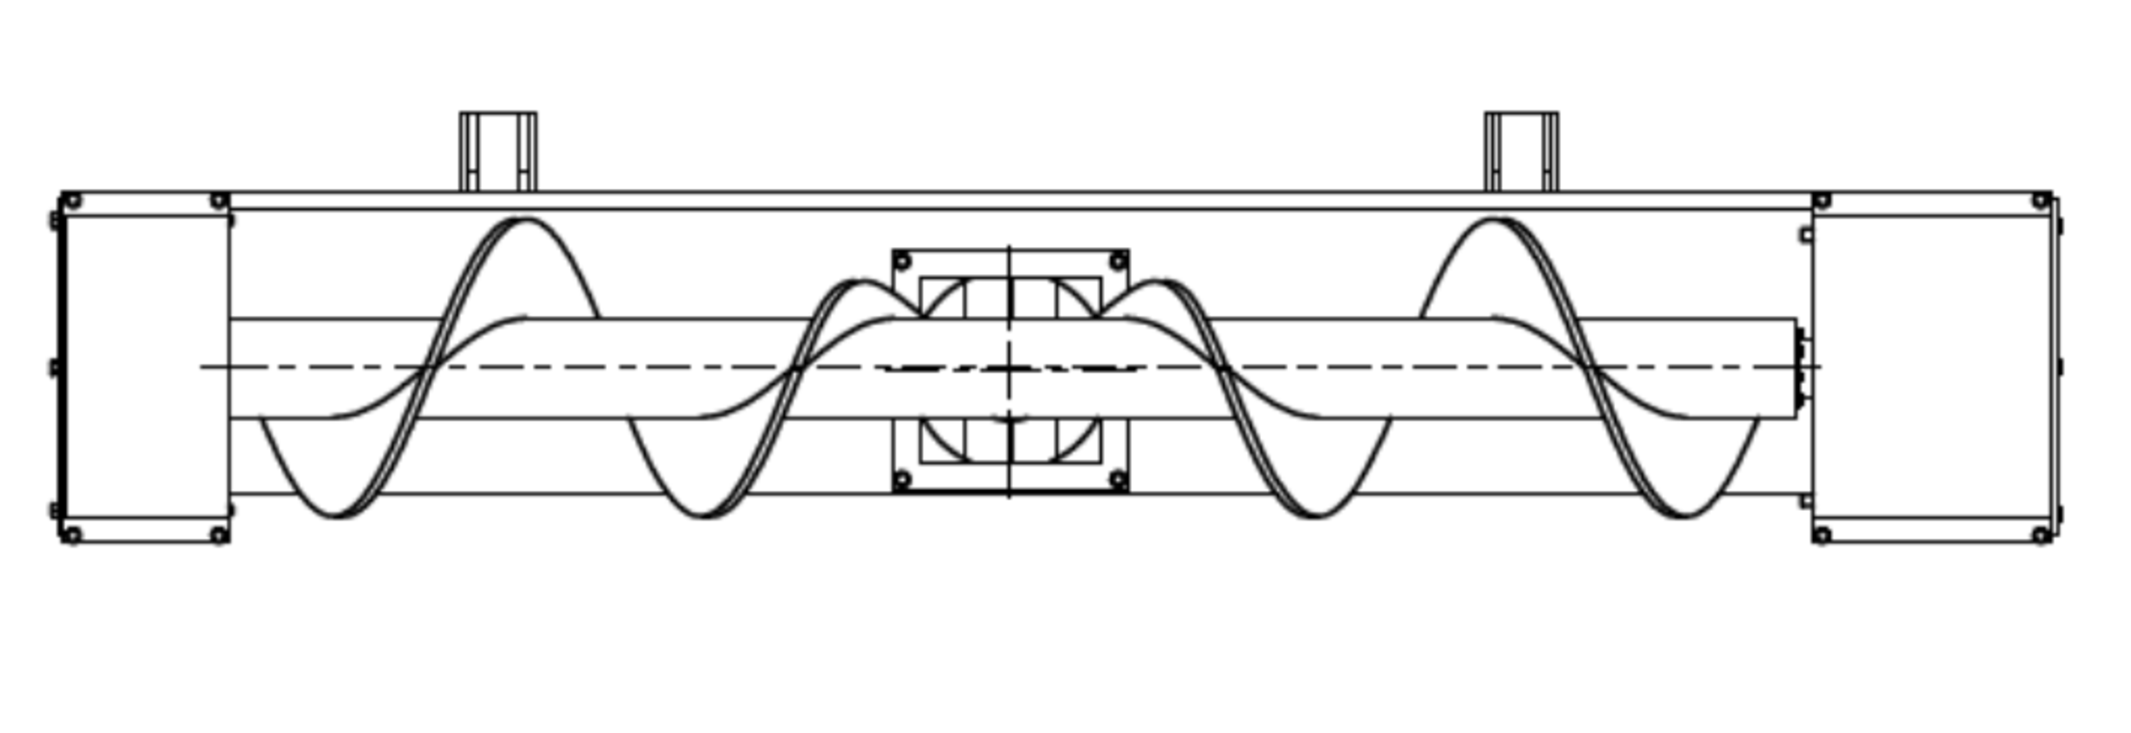
\includegraphics[width=\textwidth,trim=2 2 2 2,clip]{dredgehead.pdf}
\end{RoyalFigure}

The auger is in effect a screw conveyor which guides the material towards the suction head. \citet{perry_2007} states
that the screw conveyor is one of the oldest and most versatile conveyor types there is. It consists of a helicoid
flight mounted on a pipe which turns in a trough. Screw conveyors are well standardized,
using~\citet{international_standard_iso_neniso_1981} empirical gathered factor values for filling rates and progress
resistance.

\begin{RoyalNote}[label=assumption_dredge_speed]{ASSUMPTION}
	The assumption is made that the hydraulic system, consisting of flexible pipes and a pump, is the limiting factor in the
	mass flow, and that the auger simply delivers what is needed.
\end{RoyalNote}
